\documentclass{report}
\usepackage{graphicx}

\begin{document}
\chapter{Task 1 - Textual description of a database}
\section{Aim}

Football manager database in order to be able to simulate football manager game. \\ 
It needs to reflect realistically status, description, attributes of entities connected with football in order to ensure better simulation. \\ 


\section{Objects}
We choose miminial 5 entites to make our task easier \\ 
\begin{itemize}
    \item Player - Football players who are involved in matches, are signed to clubs, are coached by specific staff, they are the most important entity in the database as they are base for the whole database to function properly. Their behavior needs to be simulated not only during games but also after and before games.\\
    Rating for several attributes (stamina, teamwork, etc.), favourite position, reputation, contract status (is player loaned out from another club for example or maybe they do not have a club at all), injuries, retirement, age, wages, transfer value, 
    \item Club - budget (for wages, transfers), players assigned to club, staff assigned to club, competitions the club is taking part in, facilities quality (like stadium, training ground), reputation, stadium location, country of origin,
    \item Match - Clubs taking part in (from which we derivate staff and players), score, statistics (like shots on target), attendance, weather, duration (90 minutes or extended time), date, referee name,
    \item Manager - attributes (scout skills, management skills, couch skills), reputation, retirement, age, wages
    \item Competition - list of matches, schedule, clubs involved, prize, country of origin, list of stadiums, reputation (importance of the tournament)\\
    (not tournament because tournament usually refers to like cup compettions not leauge ones)
\end{itemize} 

\section{Requirements concerning data}
Player and staff attributes are between 1 and 10 \\ 
Positions are restricted to Goalkeeper, Defender, Midfield and Attacker \\ 
Reputation are restricted between 1 and 5 (as in stars with 1 between each step) \\
Quality of facilities are restricted between 1 and 5 \\ 
Type of staff - Manager, Coach, Scout, \\ 
Competition should have at least one match \\ 
Weather restricted to Sunny, Rainy, Snowy, \\ 

\section{Business Activities}
Activities we would like to cover are, players exchanged between clubs, player signed to club, player released from club (end of contract for example)
\\
clubs taking part in matches, clubs hiring players and staff, clubs taking part in competition, 
players playing in matches \\
staff being exchanged between clubs, staff signed to club, staff released from club, \\ 
Competition organizing matches

\chapter{Task 2 - ERD - Entity Relationship Diagram}
\begin{figure}[htpb]
    \centering
    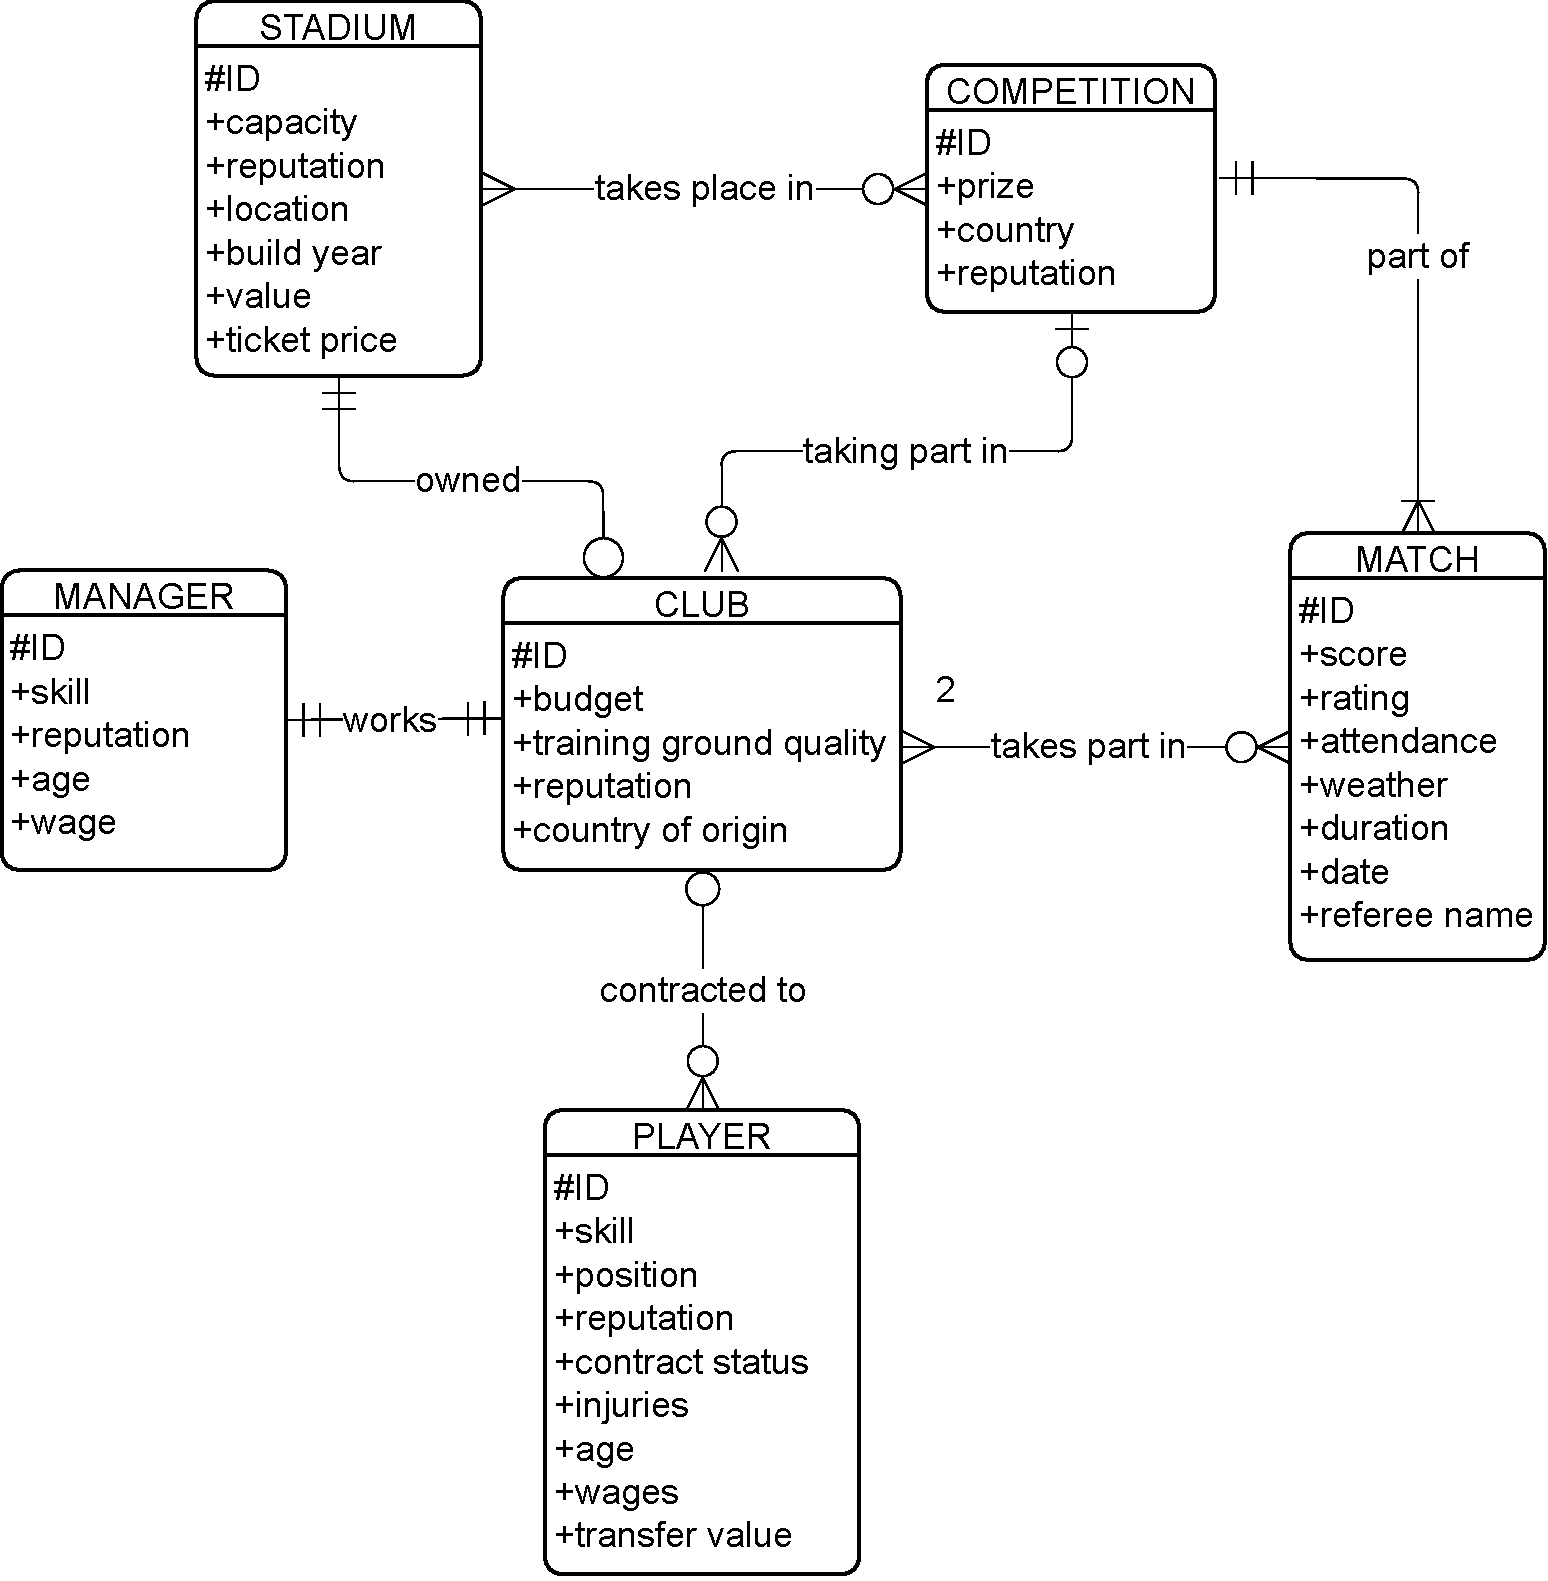
\includegraphics[width=0.8\textwidth]{erd.pdf}
    \caption{ERD}
    \label{fig:tikzpgf}
\end{figure}


\end{document}